\item A barra $AB$ de \SI{2}{\kilogram} está pendurada na posição vertical. Um bloco de \SI{1}{\kilogram}, deslizando sobre a superfície horizontal lisa com uma velocidade de \SI{3.6}{\meter/\second}, acerta a barra na sua extremidade $B$. Determine a velocidade do bloco imediatamente após a colisão. O coeficiente de restituição entre o bloco e a barra em $B$ é $e=0.8$.

\import{../answers}{answer-15}

\vspace{-1.1cm}
\begin{flushright}
	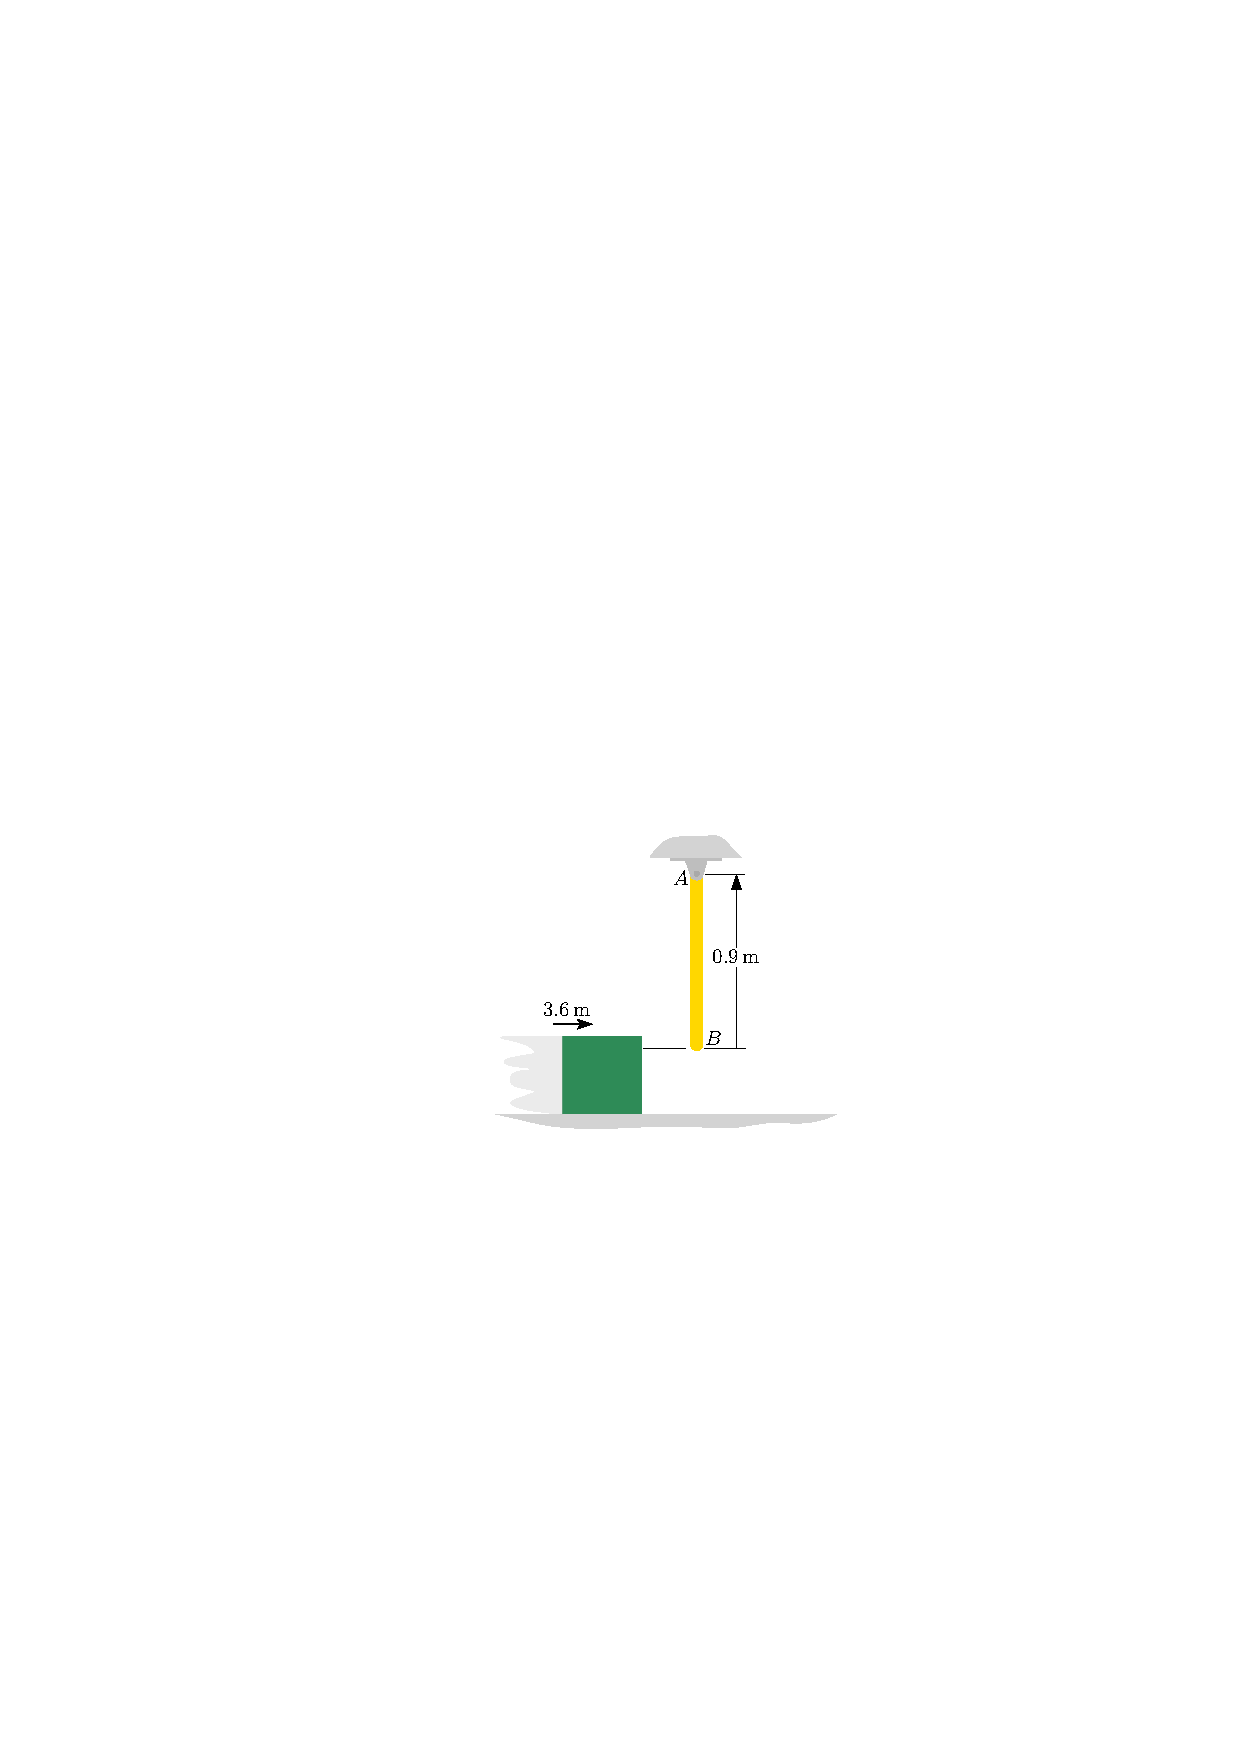
\includegraphics[scale=1.25]{../../images/draw_13}
\end{flushright}